\documentclass[a4paper]{report}

% !TEX root = .memoire/main.tex

\usepackage[utf8]{inputenc}
% \renewcommand{\familydefault}{\sfdefault}
\usepackage{geometry}
\usepackage[pdftex]{graphicx}

\graphicspath{ {./MeshlessEnKF}{./Introduction/images} {./MeshlessMethods/images} {./AlignEnKF/images} {./BiblioIntro/images} {./DataAssimilation/images}}
% \geometry{
%     left=16mm,
%     top=30mm,
%     right=16mm,
%     bottom=30mm
% }
\usepackage{appendix}
\usepackage{etoolbox}
\usepackage{xcolor}
\usepackage[absolute,overlay]{textpos}
\usepackage{lipsum}
\usepackage{array}
\usepackage{enumitem}
\usepackage{caption}
\usepackage{multicol}
\usepackage{bm}
\usepackage{amsmath}
\usepackage{amsfonts}
\usepackage{subcaption}
\usepackage[vlined, french, onelanguage]{algorithm2e}
% Hyperref setup
\usepackage[linktoc=page]{hyperref}
% \hypersetup{
%     colorlinks=true,
%     linkcolor=blue,
%     filecolor=magenta,
%     urlcolor=cyan,
%     pdftitle={Overleaf Example},
%     pdfpagemode=FullScreen,
% }
\hypersetup{
    % General settings
    pdfencoding=auto,           % Automatically handles PDF string encoding
    pdfborder={0 0 0},          % Removes borders around links
    breaklinks=true,            % Allows links to break across lines
    colorlinks=true,            % Colors the text of links and anchors
    % Link colors
    linkcolor=blue,             % Color of internal links (e.g., sections, equations)
    citecolor=green,            % Color of citation links
    filecolor=magenta,          % Color of file links
    urlcolor=cyan,              % Color of external hyperlinks
    % Metadata
    pdftitle={thesis duvillard},       % Title of the document
    pdfauthor={duvillard},              % Author of the document
    % pdfsubject={thesis},          % Subject of the document
    % pdfkeywords={keyword1, keyword2},   % Keywords for the document
    % PDF display settings
    pdfpagemode=UseOutlines,    % Opens the PDF with the bookmarks pane open
    bookmarksopen=true,         % Open the bookmarks by default
    bookmarksnumbered=true,     % Include section numbers in bookmarks
    unicode=true                % Support for non-ASCII characters in bookmarks
}
\urlstyle{same}
\setlength{\columnseprule}{0pt}
\setlength\columnsep{10pt}
\usepackage[most]{tcolorbox}
\usepackage{amsthm}
\theoremstyle{definition}
\newtheorem{definition}{Definition}%[section]

\definecolor{mycustomcolor}{RGB}{128, 0, 128}
\newcommand{\mycolor}[1]{\textcolor{mycustomcolor}{#1}}
\newcommand{\bE}{\mathbb{E}}
\newcommand{\bV}{\mathbb{V}}
\newcommand{\bC}{\mathbb{C}}
\newcommand{\nens}{N}
\newcommand{\bw}{\bm w}
\DeclareMathOperator*{\argmax}{arg\,max}
\DeclareMathOperator*{\argmin}{arg\,min}
\newcommand{\bx}{\bm{x}}
\newcommand{\mstate}{\bm{Z}}
\newcommand{\statebis}{\bm{x}}
\newcommand{\mstatebis}{\bm{X}}
\newcommand{\zz}{z_0 = 0.02}
\newcommand{\sigz}{\sigma_0^2 = 0.5}
\newcommand{\xx}{x_0 = 0.02}
\newcommand{\sigx}{\sigma_0^2 = 0.5}
\newcommand{\npart}{$N_{part} = 100$}
\newcommand{\ngrid}{$N_{grid} = 100$}
\newcommand{\sigmaY}{0.05}
\newcommand{\z}{\bm{z}}

\newcommand{\mpred}{\mathcal{Y}}
\newcommand{\mP}{\mathcal{P}}
\newcommand{\Fcorr}{\bm{F}}
\newcommand{\mdata}{\bm{D}}
\newcommand{\state}{\bm{z}}
\newcommand{\annomX}{\bm A}
\newcommand{\annomY}{\bm Y}
\newcommand{\obs}{\bm{y}}
\newcommand{\Cov}{\bm{P}}
\newcommand{\predi}{\mathcal{H} (\bm{x}_i^f)}
\newcommand{\sigmaZm}{0.5}
\newcommand{\meanZm}{\pi/2 + 0.6}
\newcommand{\bz}{\bm z}
\newcommand{\visc}{D}
\newcommand{\refv}{1.0}
\newcommand{\refvisc}{0.05}
\newcommand{\Dlow}{0.02}
\newcommand{\Dup}{0.08}
\newcommand{\vmean}{0.9}
\newcommand{\vstd}{1.2}
\newcommand{\smLow}{0.8}
\newcommand{\smUp}{1.2}

\newcommand{\by}{\bm{y}}
\newcommand{\bP}{\bm{P}}
\newcommand{\bR}{\bm{R}}
\newcommand{\bh}{\bm{h}}
\newcommand{\bd}{\bm{d}}
\newcommand{\fstate}{\bm{u}}
\newcommand{\cN}{\mathcal N}
\newcommand{\cU}{\mathcal U}
\newcommand{\cP}{\mathcal P}
\newcommand{\cV}{\mathcal V}

\newcommand{\bM}{\bm{M}}
\newcommand{\bH}{\bm{H}}
\newcommand{\bK}{\bm{K}}

\DeclareMathOperator{\Tr}{Tr}
\usepackage[most]{tcolorbox}

% Définition du modèle "boite1"
\newtcolorbox{ObjectifChap}[1][]{
    colback=blue!5!white,
    colframe=blue!75!black,
    fonttitle=\bfseries,
    title=Boîte 1,
    #1
}

% Définition du modèle "boite2"
\newtcolorbox[auto counter]{BilanChap}[1][]{
    colback=red!5!white,
    colframe=red!75!black,
    fonttitle=\bfseries,
    title=Boîte \thetcbcounter,
    #1
}
\newcommand{\norm}[1]{\left\lVert #1 \right\rVert}

\usepackage[french]{babel}
\usepackage{biblatex}
\addbibresource{biblio.bib}
% \bibliographystyle{plain}


\title{
{Méthodes d'assimilation de données pour des simulations lagrangiennes \\\
Parties contexte et méthodes particulaires}\\
{\large Ecole Polytechnique / CEA Cadarache}
}
\author{Marius Duvillard}
\date{\today}

\begin{document}

\maketitle
\tableofcontents

\chapter{Introduction}

Dans le domaine de la production d'énergie electrique, l'énergie nucléaire est une source d'énergie qui s'est imposé à de nombreux pays industrialisés.

En 2023, l'industrie électronucléaire a représenté 65\% de la production totale d'électricité en France, avec un parc composé de 56 réacteurs à eau pressurisée (REP) répartis sur 18 centrales \cite{rte2023}. Dans le monde, la production nucléaire ne fait qu'augmenter. Fin 2022, la capacité totale des 438 réacteurs nucléaires de puissance en exploitation dans 32 pays s’établissait à 393,8 gigawatts électriques (GWe). Si aujourd'hui, le nucléaire représente près de 9,8\% de la production mondiale, elle pourrait attendre 14\% du bouquet électrique en 2025 \cite{aiea2023}. D'ici 2035, le nombre de pays qui exploitent des centrales nucléaires pourrait augmenter de quelque 30\% d'ici 2050.

Le secteur est également en constante mutation avec le développement de nouvelles technologies en particulier avec les technologies de 4\textsubscript{ème} génération mais également le nouveau paradigme des SMR (\textit{Small Modular Reactor}) où la modularité permet une chaîne de déploiment et de production souple et avec une financement moindre~\cite{academie2022}.

Si ce secteur atire, c'est en particulier car il offre un très bon rapport qualité prix et est faiblement émettrice en gaz à effet de serre. Son facteur d'émission, c'est à dire la quantité d'émissions de gaz à effet de serre par unité d'énergie produite, est estimé à 12 g$CO2$eq/kWh. Il serait même encore plus faible en France~\cite{schlomer_technology-specific_nodate}. Ainsi elle est aussi émetrice que l'éolien ou bien la production photovoltaïque et est 100 à 1000 fois moins émettrice que les centrale à énergie fossiels.

L'urgence climatique pousse à considérer l'énergie nucléaire comme un levier essentiel dans la transition énergétique, offrant une alternative viable aux énergies fossiles. Cependant, cette option soulève une série de préoccupations. Outre les inquiétudes liées à la sécurité des installations et au risque de prolifération nucléaire~\cite{npt_resolution}, il est crucial d'aborder la question des déchets hautement radioactifs générés tout au long du fonctionnement des réacteurs. Chaque année, la production d'électricité entraîne la création de près de 2 kg de déchets par habitant. Une infime proportion constitue les déchets à vie longue, mais ils représentent la majorité de l'activité radioactive (0.2\% des stocks pour 95\% de l'activité). En outre, il est impératif de préserver les réserves de combustible nucléaire. Dans cette optique, les avancées technologiques telles que les réacteurs de quatrième génération visent à optimiser l'utilisation des ressources en transmutant l'uranium 238 en plutonium 239. Ainsi, la question du retraitement et de la fermeture du cycle nucléaire reste cruciale. C'est dans cette perspective que le combustible MOX (Mélange d’OXyde de plutonium et d’OXyde d’uranium) a été développé afin de recycler une partie des matières nucléaires issues du traitement des combustibles à Uranium Naturel Enrichi (UNE).

La fabrication de ce combustible passe par différentes étapes de fabrication en particulier une phase de mélange et de broyage qui a lieu au sein d'un broyeur à boulets. Ce dispositif cylindrique, rempli de boules de broyage, met en oeuvre un processus de rotation pour broyer finement le mélange de poudres d'oxyde. Sa performance est critique pour la qualité du produit final et sa sûreté d'utilisation dans les réacteurs nucléaires. Cependant, son contrôle est déterminé de manière empirique par l'expérimentateur sur une variété de paramètres tel que la vitesse de rotation, le degré de remplissage, les proportions d'alimentation et de corps broyants. Le large spectre des physiques mise en jeu à l'intérieur du tambour mais aussi le contexte de manipulation de poudres irradié rendent le contrôle et l'optimisation très complexe. Ceci a pour conséquence d’augmenter le temps de broyage, la consommation du procédé et le nombre d’intervention nécessaire sur l’installation.

C'est dans ce contexte que des outils d'aide à la compréhension par la modélisation et la simulation des étapes de la fabrication du combustible sont développées. L'objectif étant de pouvoir faire le suivi de l'état du milieu granulaire sur une large gamme de paramètre ainsi que de comprendre les mécanismes intervenant dans ce processus.

En particulier, le CEA a développé des outils pour la simulation l'état du mélange dans le milieu granulaire à l'aide de méthodes sans maillage afin de représenter.

Le problème est que ces modèles reposent toujours sur des hypothèses simplificatrices limitant leurs champs d'action. De plus, les modèles dépendent de paramètres qu'il est nécessaire de calibrer. Enfin, l'incertitude de modélisation qui en découle a pour conséquence d'augmenter l'erreur de prédiction de modèle.

Par données expérimentales nous entendons toutes données qui peut être fournies par le dispositif expérimental.

C'est ce qui justifie cette thèse, elle consiste à développer des méthodes capables de combiner les données issue de la simulation et des données exéprimentales au sein du développement du Jumeau Numérique du procédé. Le jumeau numérique est une réplique virtuelle d'un système physique, permettant de simuler, d'analyser et de prédire le comportement du système physique en temps réel. Ce modèle numérique intègre des données dynamiques et historiques, permettant une représentation précise et **synchronisée** dans le temps. Dans le contexte industriel, les jumeaux numériques utilisent l'**intelligence artificielle** (IA), l'analyse de données, et les capteurs physiques pour améliorer la compréhension des processus et faciliter la prise de décisions.


C'est dans ce contexte de la fabrication du combustible MOX (pour Mélange d’OXyde de plutonium et d’OXyde d’uranium)


\section*{Objectifs de la thèse}
% Plan de la démarche comme évoqué dans la formation.
% !TEX root = memoire/main.tex

\chapter{Contexte}

\section{Introduction}

L'objectif de ce chapitre est de présenter les différentes entitées nécessaires à la construction d'un jumeau numérique. Nous présenterons tout d'abord, quels sont les modélisations physiques utlisés pour simuler l'étape du broyeur à boulets. Nous traiterons uniquement la modélisation du mélange et de l'écoulement granulaire au sein du tambour en rotation. Dans un second temps, nous présenterons les méthodes d'acquision utilisé pour . Finalement, nous présenterons la notion de jumeau numérique et présenterons dans quel cadre observation et simulation peuvent-ils être mis en relation.

\section{Simulation de l'écoulement granulaire au sein du broyeur à boulets}~\label{sec:simu_broyeur}

\subsection{Ecoulement d'un milieu granulaire}~\label{sec:simu_granulaire}

La simulation du broyeur repose sur la représentation de l'écoulement d'un milieu granulaire. Si les écoulements granulaires sont très présents dans la nature et dans l'industrie, du fait de la nature discrète du milieu, ils sont bien moins comprise que l'écoulement d'un liquide qui se base sur les équations de Navier-Stokes.

L'écoulement granulaire va se distinguer par trois types de régime que l'on assimile généralement aux trois états de la matière: solide où où le mouvement des particules est lent et le comportement est presque statique, une couche semblable à un liquide dans laquelle les grains s'écoulent avec une certaine inertie, et une zone semblable à un gaz où les particules se déplacent à des vitesses plus élevées de manière chaotique. Ils interviennents simultanément dans l'écoulement. Ce qui complexifie sa caractérisation rhéologique.

\begin{figure}
    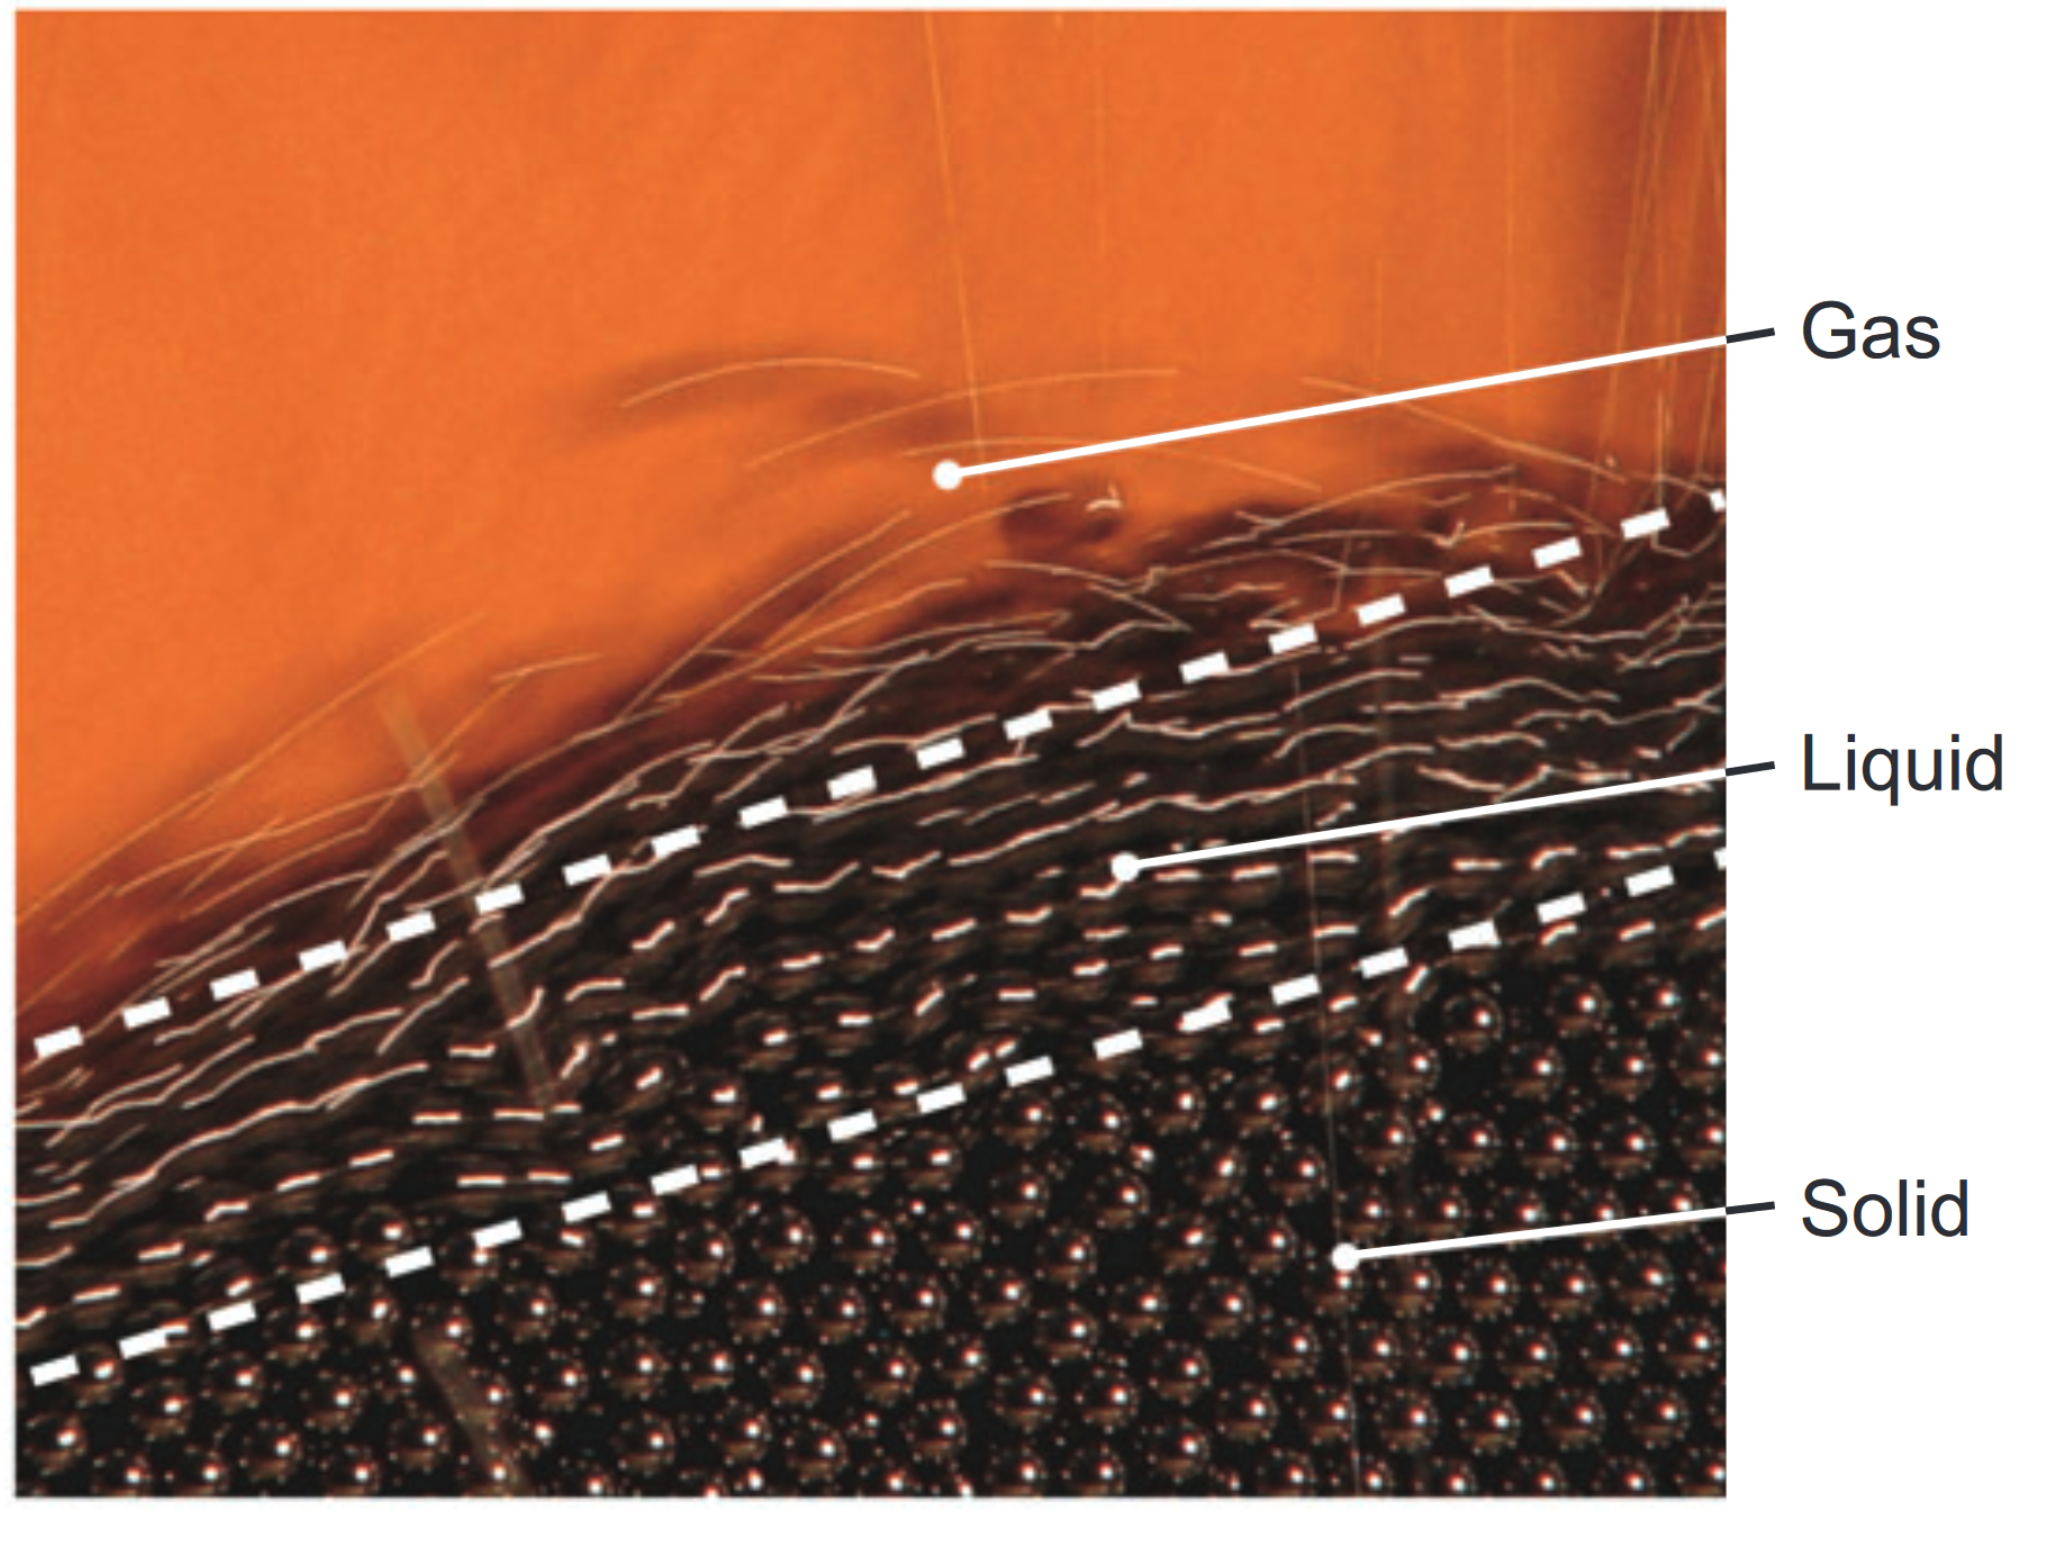
\includegraphics[width=\textwidth]{three_regimes.png}
    \caption{Image de billes d'acier s'écoulant d'un tas. Trois phases de l'écoulement granulaire, se comportant comme un gaz, un liquide ou un solide, peuvent être identifiées.~\cite{forterre_flows_2008}}
\end{figure}

Le régime solide ou frictionnel intervient en particulier en mécanique des sols pour la prédiction de la défaillance des sols pour les applications de génie civil~\cite{Campbell2006}. Dans ce cas, le critère de rupture de Mohr-Coulomb~\cite{Juvinal1991}, accompagné d'une règle de flux de la plasticité des métaux, est suffisant pour décrire le comportement de l'écoulement granulaire comme un processus continu, sans prendre en compte l'interaction des grains individuels. La loi est alors paramétré par des quantités interprétables : l'angle de friction interne, la cohésion, ainsi que l'angle de dilatation. La loi de Drucker-Prager~\cite{Drucker1952}, version lisée du critère de Mohr-Coulomb est également couremment utilisée.


Le régime liquide ou d'écoulement est principalement décrit à l'aide de lois rhéologique. Les travaux récents convergent vers une loi de comportement viscoplastique défini sous le nom de loi $\mu(I)$~\cite{gdr_midi_dense_2004,jop_constitutive_2006}. Des simulation du tambour en rotation~\cite{Cortet_2009} ont pu êter réalisé et montre une bonne correspondance pour le cas d'écoulement avec surface libre~\cite{chou_cross-sectional_2009}. Toutefois, cette loi trouve certaines limites dans le cas d'écoulement confiné où le coefficient de tassement change et où le mouvement de chaque grain entraîne des modifications significatives dans les chaînes de force. Si la prédiction est bonne au niveau des bords, elle reste toutefois insufisante au niveau des parois~\cite{Rognon_Miller_Metzger_Einav_2015}.

Finalement le régime gaz ou cinétique correspond au écoulement granulaires dispersés. Ce sont alors des modèles de cinétique des gaz qui sont utilisé pour modéliser le comportement du milieu granulaire~\cite{Ng2008}.

\subsection{Méthodes de résolution}~\label{sec:methode_resolution}

Dans le tambour en rotation l'ensemble des trois zones d'écoulement sont présentes. En fonction du nombre de Foudre, divers régimes d'écoulement apparaissent~\cite{MELLMANN2001251}. Entre autres, on retrouve le glissement, l'avalanche, la cascade, le cataracte, la centrifugation illustrés Figure~\ref{}

\begin{figure}~\label{fig:flow_drum}
    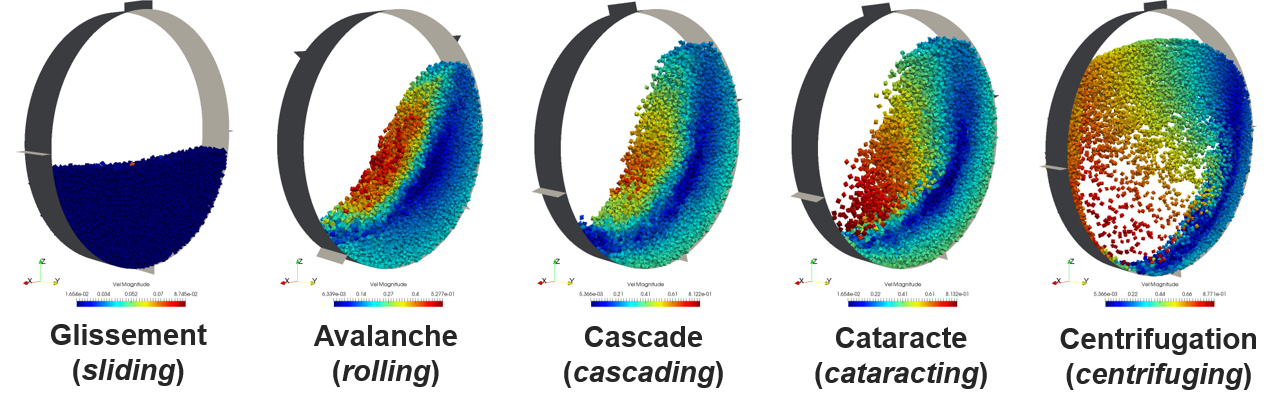
\includegraphics[width=\textwidth]{flows_in_drum.png}
    \caption{Représentation des différents régimes d'écoulement au sein du tambour en rotation avec la méthode DEM.}
\end{figure}

Ces différents régimes déterminent la qualité du mélange, du broyage. C'est en particulier le régime en cascade qui est recherché pour la réduction de taille de grain dans le broyeur à boulets. C'est dans ce régime que la surface libre prend la forme caractéristique d'un \textit{S}.

Outre la difficulté dans la définition de la loi de comportement décrit précédemment, c'est le choix de la modélisation qui est complexe pour ce type de simulation. En effet, ce problème présente un cas d'écoulement en grande transformation, avec une surface libre et nécessitant de tenir compte des interactions avec une paroi mobile voir des corps broyants.

Ce sont d'abord des lois empiriques ou analytiques qui ont été proposées dans la littérature~\cite{Ding2001,Boateng1998,Nicholas2001} mais ceux-ci sont généralement dépend du problème traité, simplifié et ne permettent donc pas une bonne généralisation.

Les méthodes de simulation ce sont à la fois portées sur des représentations continues ou discrète du milieu.

Les méthodes discrètes vont conserver une représentation particulaire du milieu en considérant un jeu de particules en équilibre. Introduite en 1979 par Cundall and Strack~\cite{cundall_discrete_1979}, la méthode des éléments discrets (DEM) a été utilisé pour la première fois pour la modélisation du tambour en rotation par Mishra and Rajamani~\cite{Mishra1992}. Ces méthodes ont l'avantage de pouvoir représenter les différents régimes d'écoulement granulaire, le mélange ou bien les phénomènes de ségrégation. On trouve également des extensions pour prendre en compte la fragmentation~\cite{orozco:hal-02409236}. Malgré ces différents avantages, la méthode DEM est très coûteuse en temps de calcul, en particulier lors de la détection des contacts. C'est d'autant plus le cas pour la simulation du tambour qui fait intervenir des grains de l'ordre du minimètre pour décrire un écoulement de l'ordre du mètre. Les grains simulés sont alors aggrandi, représentés avec des géométries plus régulière et lisse, pour permettre un temps de calcul acceptable.
De plus, la DEM nécessite l'introduction d'un terme dissipatif qu'il est souvent difficile à justifier physiquement.

De l'autre côté, les méthodes continues représentent le milieu granulaire comme un milieu continu. Le système est gouverné par les équations de conservation de masse et de quantité de mouvement. Ce type d'approche est plus à même de représenter des écoulements à grande échelle.

Dans cette famille de méthode on retrouve des méthodes qui utilise un maillage pour discrétiser les différents champs approchés. En particulier, on retrouve des méthodes utilisés en dynamique des fluides comme la méthode des volumes finis~\cite{Santos2013,arseni_granular_2020} ou bien en mécanique des solide avec des extensions de la méthodes des éléments finis comme les éléments finis eulérien~\cite{ZHENG2015361}. Si ces méthodes sont relativement plus efficaces en terme de calcul que la méthode DEM, elle ne sont pas bien adaptée aux problèmes avec des interfaces matérielles mobiles et des surfaces libres en raison de leur nature eulérienne.

Finalement, une autre classe de méthode continue a été plus récemment utilisées pour traiter des problèmes impliquant des grandes transformations, des écoulements à surface libre et des problèmes à géométries complexes. Il s'agit des méthodes sans maillage continues. Contrairement au méthode eulérienne à maillage fixe, ces méthodes dites lagrangiennes, utilise un ensemble de \textit{particulaire} comme support de discrétisation qui vont évoluer en suivant l'écoulement. De cette manière, ces méthodes ne peuvent pas souffrir de distorsion de maillage et elle sont beaucoup moins sensible à la dissipation lors de la phase d'advection. Elle permette de prendre en compte d’un mélange en affectant à chaque particules différentes particules et traite le problème de surface libre nativement. Une des plus connues est la méthode SPH (\textit{Smoothed Particle hydrodynamics}), où chaque particule transporte des quantités matérielles ainsi qu'une fonction noyau pour interpoler et discrétiser les champs continus et leurs opérateurs différentiels. Cette méthode a été utilisée pour simuler le tambour en rotation à l'aide d'une loi $\mu(I)$ couplé à une surface de charge de Drucker-Prager~\cite{zhu_lagrangian_2022}. Une autre méthode, particulièrement utilisé en mécanique des solides, est la méthode MPM (\textit{Material Point Method}). Cette dernière est une extension de la méthode PIC \textit{Particle In Cell}. Cette méthode hybride a été largement utilisée pour les écoulement granulaire~\cite{KUMAR201794} ainsi que pour la simulation du tambour en rotation~\cite{zuo_numerical_2020, chandra_nonconforming_2021} et a pu être comparé à la fois à la méthode DEM et l'expérimental pour étudier le mélange. Cependant, contrairement aux méthodes avec maillage, on perd en efficacité de calcul soit par des étapes de recherche de plus proches voisin en SPH, ou part le calcul des transfers grille/particules en MPM.

Finalement, bien que le sens physique ne soit pas le même entre méthodes discrètes et continues, il existe une prédominance des méthodes sans maillages dites particulaires pour traiter le problème de l'écoulement dans un tambour en rotation comme illustré Figure~\ref{fig:simu_granulaire}.

\begin{figure}~\label{fig:simu_granulaire}
    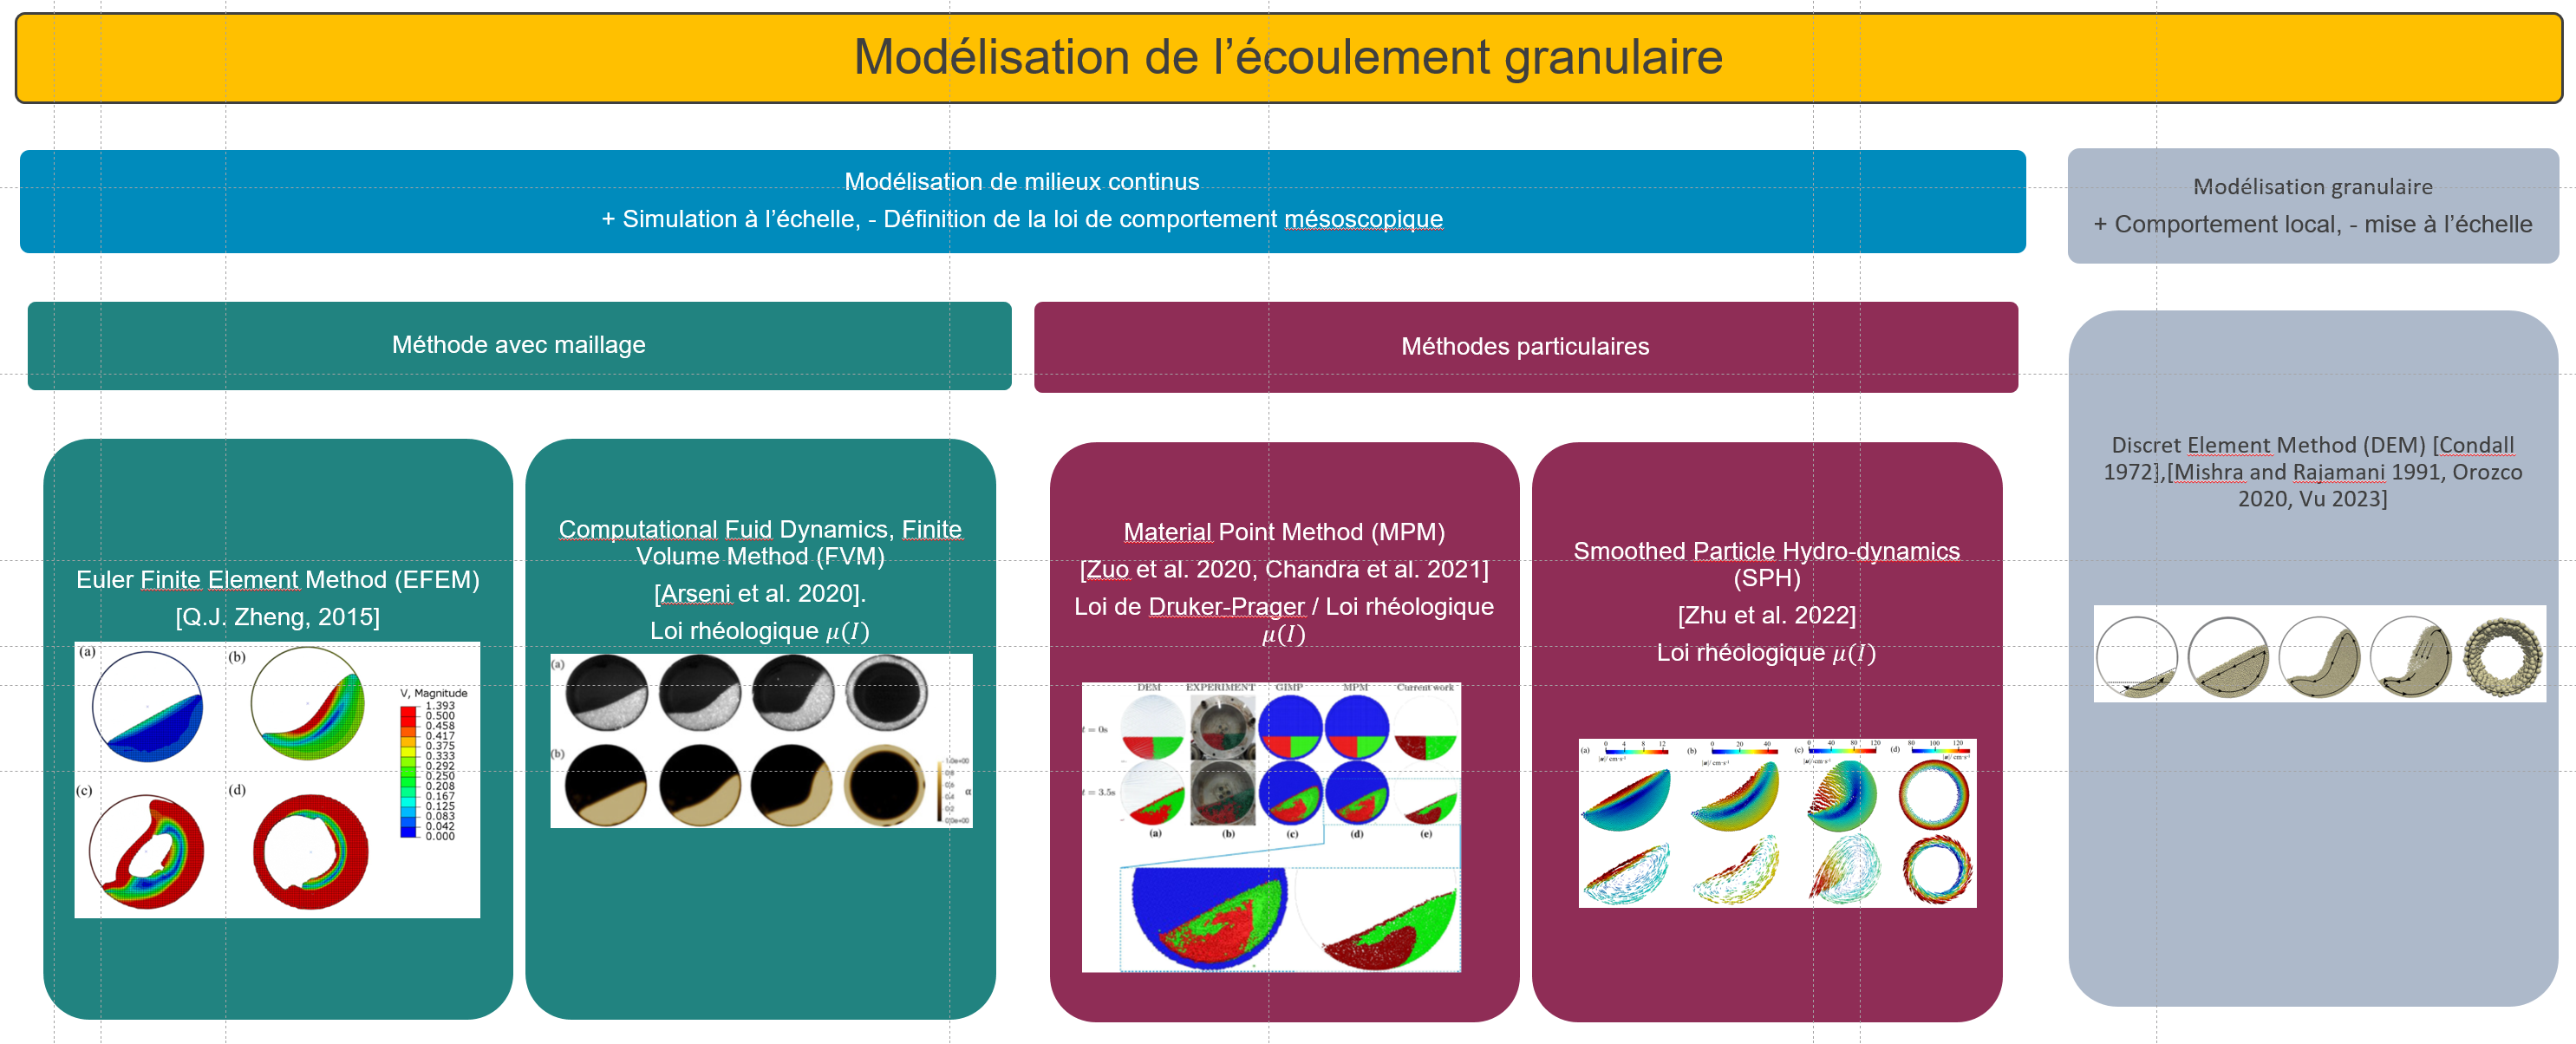
\includegraphics[width=\textwidth]{simulation_granulaire.png}
\end{figure}

\section{Mesures appliquées au tambour en rotation}~\ref{sec:mesures}

Outre l'utilisation d'outils de simulation, la validation et la compréhension du procédé se voient renforcés par l'utilisation acru de méthodes de mesure durant la phase de fonctionnement.

Ces données sont de différents types. D'une part, des données issues de l'imagerie~\cite{jarray_wet_2019,Adepu}. Celles-ci nous permetten demesurer des mesures de champ de vitesse capturées à travers la face avant d'un hublot transparent grâce à la méthode \textit{Particle Image Velocimetry} (PIV), de mesurer le ou bien de post traiter des grandeurs caractéristiques comme l'angle de repos dynamique ou de mesurer des indices de mélange.

D'autre part, des mesures accoustiques du broyeur peut révéler des informations sur divers aspects du processus, tels que les conditions de fonctionnement, les anomalies potentielles, ou encore l'usure des éléments du broyeur~\cite{Owusu, almond}.

On trouve également dans la littérature l'usage de mesure vibratoire ou de jauges de contraintes sur la paroi afin de déterminer la position du corps broyant~\cite{Davey, tano_2005}, des données issues du moteur~\cite{pedrayes_frequency_2017} ou bien l'instrumentation des boulets~\cite{Wang} (ce qui difficilement réalisable dans notre situation où la matière est contaminée).

Le laboratoire expérimental SA3E a instrumenté une maquette de broyeur dont des acquisitions sont représentées sur la Figure~\textcolor{red}{imageBastien}.

Une large gamme de mesures sont donc disponibles. Cependant, ces données mesurées ne permettent que d'avoir une représentation partielle et bruitée de l'état réel du broyage et du mélange. De plus, La qualité des résultats analysée reste néanmoins très variable. En effet, l'interprétabilité de bon nombre ce fait au travers de méthode de corrélation et non pas via des approches inductives.

Finalement, les données mesurées que nous possédons ne représentent qu'une vue brute et partielle de l'état réel, tandis que les données simulées de cet état sont sujettes à des erreurs de modélisation. Ainsi, nous souhaitons trouver un moyen d'améliorer notre connaissance des processus en tenant compte à la fois de la simulation et des mesures expérimentales.

\section{Jumeau numérique}

La notion de jumeau numérique trouve un essor considérable aujourd'hui à l'air où la données n'ont jamais été aussi présente. Le potentiel grandissant de la \textit{Big Data}, \textit{l'Internet Of Things}, le calcul haute performance (HPC) mais aussi de l'intelligence artificiel (IA) et en particulier l'apprentissage profond ouvre la voie à de nouveaux outils. Bien que sur toutes les lèvres, on trouve difficilement une définition univoque de ce paradigme.
En effet, le jumeau numérique peut être tour à tour vu comme un réplique haute fidélité capable d'émuler un système réel~\cite{noauthor_digital_nodate}, ou bien comme un modèle dynamique qui est capable d'être mis à jour avec les données de son pendant physique au long de son cycle de vie afin d'apporter une aide à la décision~\cite{AIAA2020}. Pour éviter toute confusion la distinction est souvent faite entre \textit{Virtual Twin}, \textit{Predictive Twin}, ou encore \textit{Twin Projection}~\cite{Kvamsdal}.

En définitif, le jumeau numérique n'est autre qu'un modèle, et répond au principe d'utilité énoncé par Box~\cite{box1979}: \textit{All models are wrong, some are useful}.

Le jumeau numérique pour l'étape de fabrication du combustible peu donc répondre à différents niveaux d'usages comme :
\begin{itemize}
    \item avoir une meilleure compréhension du procédé ;
    \item avoir une prédiction fidèle de l'état du système ;
    \item proposer une optimisation des paramètres de contrôle ;
    \item surveiller l'état du procédé dans une optique de maintenance prédictive ;
    \item contrôler la qualité du produit.
\end{itemize}

Finalement, le jumeau numérique peut être formalisé mathématiquement sous la forme d'un modèle graphique probabiliste proposée par Kapteyn et al.~\cite{kapteyn_probabilistic_2021}.
Elle permet de relier de bout en bout les flux de données entre capteur, et modèle numérique, mais aussi avec les paramètres de contrôle et de récompense. La représentation graphique du jumeau numérique du broyeur est présentée en Figure~\ref{fig:graph_dt}.

\begin{figure}~\label{fig:graph_dt}
    \centering
    \begin{subfigure}{0.49\textwidth}
        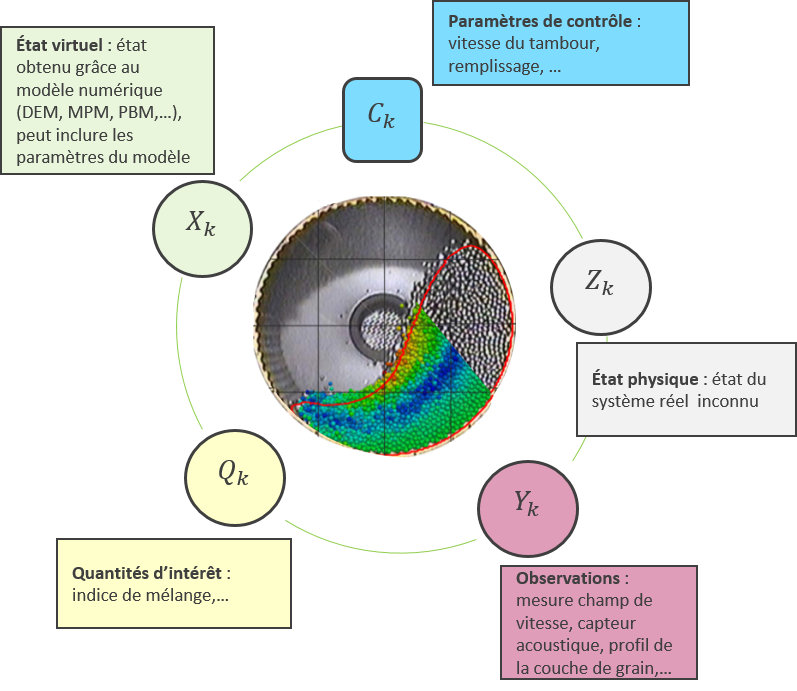
\includegraphics[width=\textwidth]{dt_broyeur.png}
    \end{subfigure}
    \begin{subfigure}{0.49\textwidth}
        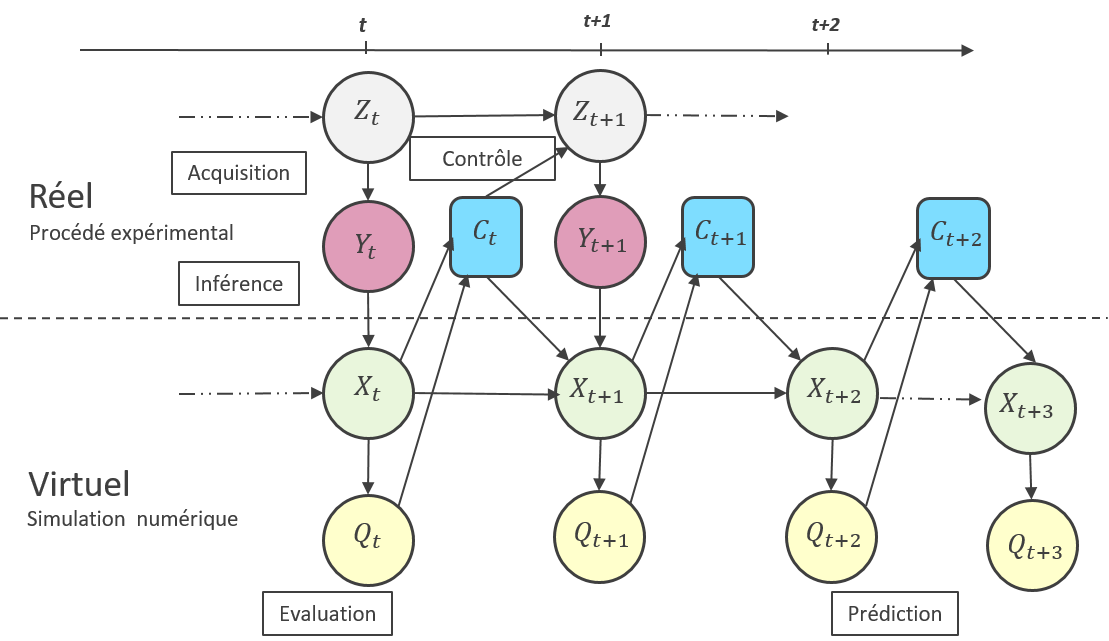
\includegraphics[width=\textwidth]{dt_seq.png}
    \end{subfigure}
\end{figure}

D'une part, on représente bien l'entité réel qui n'est connue qu'au travers des observations présentées Section~\ref{sec:mesures}. Mathématique il s'agit d'un modèle de Markov caché. D'autre part, on retrouve le modèle virtuel qui permet d'avoir accès aux variables d'intérêt et de prédire l'évolution de l'état du système à l'aide des modèles physiques comme présenté en Section~\ref{sec:simu_broyeur}
Finalement, on remarque le lien d'inférence qui permet de relier les observations et avec l'état virtuel du système. Fondamentalement, ce sont les méthode d'inférence bayésienne, et l'assimilation de données qui sont utilisés à cette étape.
Le modèle probabiliste permet ainsi d'intégrer dans la construction du jumeau numérique la notion de quantification d'incertitude.

\section{Bilan du chapitre}

Ce chapitre nous a permis de montrer la prédominance et des méthodes sans maillage pour simuler le mélange dans un tambour en rotation. Il a permis de présenter un large spectre de méthodes d'acquisition. Finalement, il a permis de présenter le jumeau numérique comme un modèle dynamique capable d'intégrer les données issues de l'observation. Ce lien est possible au travers de méthodes d'assimilation de données.






\chapter{Outils et méthodes}
% !TEX root = main.tex

\chapter{Simulation du tambour et Assimilation de données}

Nous avons vu dans le chapitre précédent que l'assimilation dépendait de la définition d'un modèle et de son état pour définir le prior et la vraissemblance. Les simulations de l'écoulement dans le broyeur à boulets qui reposent sur des discrétisations sans maillage dites particulaires, définissent ainsi notre état et son modèle d'évolution. Cependant, le caractère Lagrangien de la définition de l'état implique d'évaluer jusqu'à quel point les méthodes classiques d'assimilation peuvent être adaptée. En effet celles-ci se base sur des états dont la discrétisation restent identique. De plus, le fait que l'espace soit continu ou discret va également modifier la signification de l'état et sa capacité à être mis à jour.
Dans cette partie, nous reprendrons les principales familles de formulation particulaire en développant les formulations des méthodes DEM, SPH et MPM.  Pour chacune d'entre elles, nous évoquerons les sigularités et limites à l'adaptation des méthodes d'assimilation de données. De plus, nous présenterons la Méthode Vortex comme une méthode particulaire modèle pour la suite manuscrit.


\section{Méthode des éléments discrets (DEM)}

La méthode consiste à considérer le mouvement d'un ensemble de $N$ grains composant le milieu. Celui-ci est décrit par l'équation de la dynamique qui peut s'écrire sous la forme

\begin{equation*}
    \left\{
    \begin{aligned}
         & m_{i} \frac{ d^{2}\vec{r}_i }{dt^2}=\vec{f}_{i},\; i=1\ldots N      \\
         & I_{i} \frac{d \vec{\omega}_{i}}{dt}=\vec{\Gamma}_{i},\; i=1\ldots N
    \end{aligned}
    \right.
\end{equation*}où $`N`$ est le nombre de grains, $`m_{i}`$ est la masse, $`I_i`$ est le moment d'inertie, $`\vec{r}_{i}`$ est la position, $`\vec{\omega_{i}}`$ est la rotation, $`\vec{f}_{i}`$ est la force exercée sur le grain considéré et $`\vec{\Gamma_{i}}`$ le moment associé à la force $`\vec{f}_{i}`$.

La force $`\vec{f}_{i}`$ peut être décomposée de la manière suivante

\begin{equation*}
    \vec{f}_{i}=\underset{{\scriptstyle j\neq i}}{\sum}\vec{f}^{c}_{ij}+\vec{f}_{ext}
\end{equation*}

où $`\underset{{\scriptstyle j\neq i}}{\sum}\vec{f}^{c}_{ij}`$ représente les forces de contact qui s'exercent à la surface de la particule $i$ et les forces externes $`\vec{f}_{ext}`$ sont celles appliquées au centre de la particule $`i`$ (par exemple la force de gravité).

Les forces de contact sont décrite par des loi de contact entre les grains ainsi qu'entre les grains et la paroi. Dans le cas élastique, la modèle de Hertz est adapté pour décrire l'intéraction normale. Le modèle Hertz-Mindlin permet de déterminer les interactions tangentielles élastiques. Ces loi sont fonctions de l'interpénétration inter-particule et de la vitesse relative interpaticules. Par exemple, dans le cas de particules sphérique l'interpénétration est défini comme $\delta_{ij} = \norm{\bm x_i - \bm x_j} - (R_i - R_j)$ où $x$  est la position et $R$ le rayon d'une particule.

La force de contact tend à pénaliser l'interpénétration via des coefficients de raideur $k$ et d'amortissement $\gamma$ qui dépendent des propriétés mécaniques des grains de de la paroi. Il existe plusieurs algorithme pour résoudre numériquement les équations de la dynamique. Le plus utilisé est l'algorithme de Verlet en vitesse.


La méthode des éléments discrets (DEM, pour Discrete Element Method) est une technique de simulation numérique utilisée pour étudier le comportement des systèmes de particules, tels que lors du mélange broyage à l'intérieur du broyeur à boulets. Cette approche est particulièrement pertinente pour modéliser les interactions complexes entre les particules dans ces systèmes, où la dynamique individuelle de chaque particule peut avoir un impact significatif sur le processus global.

Dans un mélangeur-broyeur, les particules interagissent entre elles, avec les parois du broyeur, et avec le corps broyant. La DEM modélise chaque particule individuellement, en tenant compte de ses propriétés physiques telles que la taille, la forme, la masse, la rigidité, et le modèle de fragmentation. Les interactions incluent les forces de contact, les forces de frottement, et les forces de cohésion.

Le processus de simulation DEM dans un mélangeur-broyeur commence par la définition des propriétés des particules et des conditions initiales du système. Le mouvement de chaque particule est ensuite calculé en résolvant les équations de Newton pour le mouvement et la rotation. Ces calculs tiennent compte des forces et des moments résultant des collisions et des interactions entre particules, ainsi que de l'interaction des particules avec les parois du broyeur.

L'un des principaux avantages de la DEM est sa capacité à fournir des informations détaillées sur le mélange et le broyage des particules à l'échelle microscopique. Elle permet d'analyser comment les variations dans la configuration des particules, la vitesse de rotation du broyeur, et d'autres paramètres opérationnels influencent l'efficacité du broyage et l'homogénéité du mélange.

Cependant, l'utilisation de la DEM pour la simulation de mélangeurs-broyeurs peut être exigeante en termes de ressources informatiques, en particulier pour les systèmes avec un grand nombre de particules.


\subsection{DEM et assimilation de données}

L'assimilation de données, lorsqu'appliquée à des systèmes simulés par la méthode des éléments discrets (DEM), se heurte à plusieurs limites importantes présentées ci-dessous.

\subsubsection{Limites de la DEM avec les méthodes variationnelles}

Dans le cadre des méthodes variationnelles d'assimilation de données, telles que 3D-Var, le principal défi est la grande dimensionnalité du problème d'optimisation.
En effet, La DEM simule le comportement de chaque particule individuellement. Cela signifie que l'état du système comprend les variables cinématique de chacune d'elles : position, la vitesse, accélération mais aussi la position angulaire, la vitesse angulaire et l'accélération angulaire ou la densité de chaque particule. Pour un système avec des milliers voire des millions de particules, cela conduit à un problème d'optimisation de très grande dimension.

De plus, il existe un nombre extrêmement élevé de contraintes, notamment l'interdiction de l'interpénétration des particules. Ces contraintes doivent être prises en compte pour assurer que la solution d'optimisation soit physiquement admissible.

L'application des méthodes 3D-Var et 4D-Var est donc trop exigeante d'un point de vue des temps de calcul.

De plus, les filtres variationnels corrigeant des erreurs d'intensité selon des normes euclidiennes, la variation selon les positions des observations ne sera pas linéaire.

Ainsi, la définition d'un état de particules discrètes implique de résoudre un problème d'optimisation non-linéaire de grande dimension.

\subsubsection{Limites de la DEM avec EnKF}
Pour l'EnKF, l'état estimé du système est une combinaison linéaire des états prédits par les différents membres de l'ensemble. Cependant, dans le contexte de la DEM, cette combinaison linéaire des états n'est pas nécessairement physiquement admissible. Par exemple, elle pourrait conduire à des situations où les particules s'interpénètrent ou violent d'autres lois physiques.
En d'autres terme, la mise à jour ne peut être réalisé que via le solveur lui-même capable de vérifier des contraintes de non interpénétrabilité mais ne peut être réalisé directement.

Un autre problème avec l'EnKF dans le contexte de la DEM est la difficulté de faire correspondre les particules entre les différents membres de l'ensemble. Même si initialement chaque membre possèdait la même configuration particulaire mais avec des propriétés différentes, chaque particule a sa propre trajectoire unique en cohérence avec les intéractions dans son voisinage. Aligner ces trajectoires à travers les différents membres de l'ensemble pour une assimilation de données cohérente est un défi complexe. Cette difficulté est exacerbée par le nombre élevé de particules et par la nature dynamique et chaotique de leurs interactions.

Dans le cas pus général où les membres n'aurait pas le membre de particule la correspondance des états est d'autant plus complexe.

Ainsi, le caractère discret de la méthode DEM rend l'assimilation par EnKF à la fois complexe par :

\begin{itemize}
    \item une définition de l'état et de ses statistiques non univoque ;
    \item la construction du gain de Kalman d'Ensemble ;
    \item la contrainte d'interpénétration lors de la mise à jour.
\end{itemize}

\section{Méthodes particulaires continues}
\subsection{Méthodes basées sur les particules}~\label{Background_Part}
Nous envisageons des méthodes par particules pour résoudre des problèmes continus en mécanique des fluides ou des solides. Cela inclut des méthodes telles que l'hydrodynamique par particules lissées (SPH) \cite{lucy_1977,gingold_monaghan_sph_1977} et la méthode des vortex (VM) \cite{cottet_vortex_2000}, et s'étend à d'autres méthodes comme la méthode des points de matériau (MPM) \cite{sulsky_particle_1994}. Elles partagent toutes de décomposer cette fois le domaine en un ensemble $\mathcal{P}$ de particules qui suivent la dynamique du problème. Ainsi, la discrétisation suit la transformation appliquée au milieu en transportant des quantités attachées à chaque particule. Elles sont en cela des méthodes Lagrangienne.

\subsubsection{Discrétisation par particules}

La solution représentée par le jeu de particule est obtenue grâce à deux éléments: une appproximation grâce à un noyau de lissage et l'approximation particulaire d'un opérateur intégral. Si la représentation de la solution peut évoluer suivant la méthode (en particulier avec la méthode MPM), la solution peut toujours être exprimé de cette manière suivant le choix du noyau.

Tout champ relativement régulier $\bm{u}$ sur $\Omega$ peut être écrit grâce à la propriété de filtrage de Dirac

\begin{equation*}
    \bm{u}(\bm{z}) = \int_{\Omega} \bm{u}(\bm{z'}) \delta(\bm{z'} - \bm{z})  d\bm{z'},
\end{equation*}avec $\delta$ la distribution de Dirac.

Une fonction de noyau $\phi_\varepsilon$ est introduite pour obtenir une estimation moyenne $\langle \bm{u} \rangle$ de $\bm{u}$ telle que

\begin{equation*}
    \langle \bm{u}(\bm{z}) \rangle = \int_{\Omega} \bm{u}(\bm{z'}) \phi_\varepsilon(\bm{z}-\bm{z'}) d\bm{z},
\end{equation*}où $\varepsilon$ est la longueur de lissage. Le noyau lisse doit au moins respecter les propriétés suivantes

\begin{eqnarray*}
    && \int_{\Omega} \phi_\varepsilon(\bm{z}) d\bm{z} = 1,      \\
    && \phi_\varepsilon(\bm{z}) \to \delta(z), \quad \varepsilon \to 0, \\
    && \phi_\varepsilon(\bm{z}) \in C^k,  \quad k \geq 1,
\end{eqnarray*} où les deux premières propriétés sont des propriétés résiduelles de la distribution de Dirac et la dernière est une exigence de différentiabilité nécessaire pour approcher les opérateurs différentielles.

La fonction moyenne $\langle \bm{u} \rangle$ est ensuite utilisée pour approximer la fonction d'origine.

Dans un second temps, le domaine d'origine $\Omega$ est subdivisé avec $N_p$ sous-domaines $\Omega_p$ associés à une particule Lagrangienne à l'emplacement $z_p \in \Omega_p$. Nous notons $V_p$ le volume de $\Omega_p$. Cette discrétisation est ensuite utilisée pour approximer la fonction moyenne de telle sorte que

\begin{eqnarray*}~\label{part_approx}
    \langle \bm{u}(\bm{z}) \rangle &=& \sum_p \int_{\Omega_p} \bm{u}(\bm{z'}) \phi_\varepsilon(\bm{z}-\bm{z'}) d\bm{z'} \\
    &\approx& \sum_p \bm{u}(\bm{z}_p) V_p \phi_\varepsilon (\bm{z}-\bm{z}_p) \\
    &\approx& \sum_p \bm{U}_p \phi_\varepsilon (\bm{z}-\bm{z}_p).
\end{eqnarray*}

Ainsi, toute fonction définie sur une discrétisation par particules est définie par un ensemble de positions de particules $\bm{z}_p$ associées à une valeur de particule $\bm{U}_p = \bm{u}(z_p) V_p$ et un noyau lisse $\phi_\varepsilon$.

Sur la base de cette discrétisation, l'opérateur différentiel peut être dérivé à travers cette formulation.

Tout comme le champ $\bm u$, la même interpolation peut être appliquée pour obtenir

\begin{equation*}
    \nabla \bm{u}(\bm{z}) = \sum_p \bm{U}_p \nabla \phi_\varepsilon (\bm{z}-\bm{z}_p).
\end{equation*}

Ils existent toutefois une grande variété de formule pour approximer l'opérateur gradient. Dans ces cas, ce sont les propriétés de conservation associées au champ qui sont privilégiées.
Généralement, un terme additionnel est introduit lorsque le champ est évalué à la position d'une particule $q$ tel que

\begin{equation*}
    \nabla \bm{u}(\bm{z}_p) = \sum_q (\bm{U}_q - \bm{U}_p) \nabla \phi_\varepsilon (\bm{z_q}-\bm{z}_p)
\end{equation*}, où $\sum_q \bm{U}_p \nabla \phi_\varepsilon (\bm{z_q}-\bm{z}_p)$ est nul par propriété de localisation du noyau $\phi_\varepsilon$.

\subsubsection{Exemple de fonctions de noyau}

Plusieurs noyaux ont été utilisés en fonction de la méthode. La formulation originale de la MPM n'utilisait pas de noyau de substitution et écrivait la densité comme suit

\begin{equation*}
    \bm{u}(\bm{z}) = \sum_p \bm{U}_p \phi_\varepsilon (\bm{z}-\bm{z}_p)
\end{equation*}

Et la résolution est basée sur une projection sur une grille de fond associée à certaines fonctions de forme \cite{sulsky_particle_1994}.

La méthode GIMP est une formulation différente qui utilise la fonction de Heaviside \cite{bardenhagen_generalized_2004} et associe donc un volume autour de chaque particule

\begin{equation*}
    M_1(r) = \frac{\alpha}{\varepsilon}\left\{\begin{aligned}
         & 1; & r \leq \varepsilon \\
         & 0; & \text{sinon}
    \end{aligned}
    \right.
\end{equation*}où $r = \norm{\bm{z}}_2$.

Cette méthode a été introduite pour éviter le problème de passage de cellule lorsque une particule se déplace d'une cellule à une autre à travers la grille de fond.

Dans la méthode SPH, comme son nom l'indique, un noyau lisse est associé pour approximer la solution. Théoriquement, il pourrait s'agir de la fonction de noyau gaussien

\begin{equation*}
    \phi_g(r) = \frac{1}{{(\pi \varepsilon^2)}^{d/2}} \exp(-r^2/\varepsilon^2)
\end{equation*}.

Ce noyau est infiniment différentiable mais défini sur un support non compact. En pratique, nous utilisons une coupure pour supprimer les valeurs négligeables pour une grande distance par rapport à une particule.

D'autres noyaux, basés sur des fonctions B-Spline pour travailler sur un support compact. Ces fonctions sont également positives, ce qui est une exigence pour certains champs comme la densité.

Par exemple, le B-spline quadratique, que nous appelons $M_3$, est défini avec
\begin{equation}~\label{quadratic_kernel}
    M_3(r) = \frac{\alpha}{\varepsilon^d}\left\{ \begin{aligned}
         & \frac{3}{4} - |q|^2                            & 0 \leq           & |q| < \frac{1}{2} \\
         & \frac{1}{2} {\left(\frac{3}{2} - |q|\right)}^2 & \frac{1}{2} \leq & |q| < \frac{3}{2} \\
         & 0                                              & \frac{3}{2} \leq & |q|
    \end{aligned}
    \right.
\end{equation}avec $r = \norm{z}_2 $ et $q = r / \varepsilon$ et $\alpha$ la condition de normalisation et $d$ la dimension spatiale.

Ce noyau garantit la continuité $C^1$.
Le noyau cubique est un autre noyau B-Spline qui est
\begin{eqnarray}~\label{cubic_kernel}
    M_4(r) &=&  \frac{\alpha}{\varepsilon^d} \left\{ \begin{aligned}
         & \frac{1}{6}{(-|q|+2)}^3 - \frac{4}{6}{(-|q|+1)}^3 & 0 \leq      & |q| \leq  1 & \\
         & \frac{1}{6}{(- |q|+2)}^3                          & 1      \leq & |q| \leq 2  & \\
         & 0                                                 & 2 \leq      & |q|
    \end{aligned}
    \right.
\end{eqnarray}

Dans ce dernier cas, le facteur de normalisation $\alpha$ est

\begin{equation*}
    \alpha = \left\{ \begin{aligned}
         & 1;    \quad      & 1\text{ d} \\
         & 30/14 \pi; \quad & 2\text{ d} \\
         & 3/ 2\pi; \quad   & 3\text{ d}
    \end{aligned}
    \right.
\end{equation*}

Notez que ces noyaux ont été définis avec la coordonnée radiale $r$. Une autre possibilité serait de définir le noyau multidimensionnel comme le produit tensoriel du noyau 1D

\subsection{SPH}

La méthode SPH a étét développée indépendemment par Lucy~\cite{lucy_1977}, et Gingold et Monhagan~\cite{gingold_monaghan_sph_1977}. Elle a été formulé initialement pour dess problème de formation et d'évolution des systèmes stellaires. Tout comme en mécanique quantique sont but est de réprésenter le système discret en le lissant pour obtenir un milieu continu discrétisé par un ensemble de particules. En mécanique, cette méthode est vu comme une méthode de discrétisation sans maillage d'un milieu continu.
Elle consiste à résoudre la forme forte des équations de la dynamique en approchant les champs et les opérateurs différentiels à l'aide de l'approximation particulaire et l'approximation par noyau précédemment évoqué.

Les équations résoluent sont l'équation de continuité et l'équation de conservation de la quantité de mouvement à travers l'équation d'Euler

\begin{eqnarray*}
    \frac{d\rho}{dt} + \rho \nabla \cdot \bm{v} = 0, \\
    \frac{d\bm v}{dt} = \frac1\rho \nabla \cdot \bm \sigma,
\end{eqnarray*}où $\rho$ est la densité, $\bm v$ la vitesse, $\bm \sigma$ la contraite de Cauchy.

En utilisant la règle d'approximation du gradient le terme $\rho \nabla \cdot \bm{v}$ peut être approximé pour chaque particule, ce qui donne pour l'équation de continuité

\begin{equation*}
    \frac{d\rho_p}{\sum_{q} m_j (\bm v_j - \bm v_i) \cdot \nabla \phi_\varepsilon(\bm z_p - \bm z_q)}.
\end{equation*}

De la même manière, l'équation d'équilibre des quantités de mouvement peut êter discrétisé. La forme suivante est généralement utilisée

\begin{equation*}
    m_p \frac{d \bm v}{dt} = \sum_{q} m_p m_q \left(\frac{\bm \sigma_p}{\rho_p^2} + \frac{\bm \sigma_q}{\rho_q^2} \right) \cdot \nabla \phi_\varepsilon(\bm z_p - \bm z_q).
\end{equation*}

Cette version est symétrique par rapport aux indices $p$ et $q$ ce qui favorise les propriétés de conservation.

Finalement, les équations de la dynamique sont intégrées dans le temps généralement à l'aide d'un algorithme dit \textit{leap-frog}.

\section{Méthode des points matériaux (material point method, MPM)}

La méthode des points matériaux (MPM) est une technique de simulation numérique innovante, particulièrement adaptée à la modélisation de phénomènes complexes comme ceux rencontrés dans les mélangeurs-broyeurs. Cette méthode représente un compromis entre les approches par éléments finis et par particules, offrant ainsi une modélisation efficace des interactions matérielles dans des environnements dynamiques et déformables.

Dans la MPM, l'intérieur du tambour d'un mélangeur-broyeur est conceptualisé comme un milieu continu, adoptant une perspective macroscopique. La réponse du milieu est alors représenté par une loi de comportement mécanique telle que la loi de Drucker-Prager. Cela contraste avec la méthode des éléments discrets (DEM), qui se concentrent sur les interactions particule-par-particule.

Le processus de simulation avec la MPM implique des itérations entre une grille de calculs et des particules matérielles. Chaque particule porte des informations essentielles associées au matériau, telles que la masse, le volume, et les propriétés mécaniques (variables internes, gradient de déformation...). Ces particules sont utilisées pour transférer des informations sur et hors d'une grille de calculs, où les équations de mouvement et de comportement du matériau sont résolues.

Cette approche hybride permet à la MPM de capturer efficacement les déformations importantes, les ruptures, et d'autres comportements complexes du milieu qui sont fréquents dans les opérations de mélange et de broyage. En revanche, la description fine du phénomène proposée par la DEM n'est plus disponible.

En termes de temps de calculs, la MPM est plus efficace que la DEM.

\subsection{La MPM et la DA}
La MPM offre un cadre exploitable pour mettre en place une méthode de DA.
La structure de grille sous-jacente à la MPM permet une modélisation l'utilisation des méthodes variationnelles ou des méthodes d'ensemble. La structure de particules est aussi plus flexible dans le sens où elles représentent une densité de matière : elles peuvent donc s'interpénétrer.

\subsubsection{MPM et méthodes variationnelles}
Le principal défi est de gérer la dimension du problème d'optimisation pour la 3D-Var, ainsi que construire un modèle adjoint pour la 4D-Var.
Deux pistes sont envisageables : mettre à jour les champs nodaux et les champs particulaires. Comparativement à la DEM, le nombre de variables et le nombre de contraintes sont drastiquement réduits au prix d'une représentation plus grossière.

\subsubsection{MPM et EnKF}
Pour l'EnKF, l'état estimé est une combinaison linéaire des états prédits. Dans le contexte de la MPM, cela signifie que la mise à jour de l'état peut être directement effectuée sur la grille de calcul, plutôt que sur les particules individuelles. Cette approche réduit la complexité des calculs et facilite l'assimilation de données dans des systèmes à grande échelle.

Cependant, l'intégration de la MPM avec l'EnKF soulève plusieurs questions importantes :

1. **Transfert d'Informations de Particules à la Grille** : La première question concerne le transfert efficace des informations des particules vers la grille. Cela nécessite des algorithmes précis pour garantir que les informations pertinentes sur les propriétés des matériaux, telles que la densité, la contrainte, et le gradient de déformation déformation, sont correctement représentés sur la grille de calcul.

2. **Remaillage de Particules pour Représenter l'État Mécanique** : Une autre question clé est de savoir comment effectuer un remaillage des particules pour représenter fidèlement l'état mécanique du système après assimilation. Cela est crucial pour maintenir la cohérence et l'exactitude du modèle MPM, en particulier après des mises à jour successives de l'état du système.

Au travers des précédentes méthodes particulaires, nous constatons que l'application des méthodes d'assimilation sont innégalement applicable. En particulier, les méthodes discrètes n'offre pas la possibilité de corriger directement l'état de la discrétisation, mais nécessite une correction au travers du schémas d'intégration. D'autre part, les méthodes particulaires continues (par exemple MPM, SPH), permettent de modifier et faire varier dans son intégralité la discrétisation particulaire. En effet, chaque particule est définie en un point, ce qui annule tout problème d'interpénétration. Toutefois, il reste nécessaire de définir les
Afin de facilité le développement de nouveaux filtres, une autre méthode particulaire a été utilisée la méthode Vortex. Elle a été choisie car elle offre une modélisation plus simple que les méthodes SPH et MPM. En effet, chaque particule ne transporte qu'une quantité scalaire.Toutefois, elle dispose de toutes les caractéristiques d'une méthode particulaire continue. On retrouve de plus différentes version de cette méthode. Ainsi, la formulation classique de la méthode se rapproche de la méthode SPH et la méthode Vortex-In-Cell de la méthode MPM en mécanique des solides.

\section{Méthode Vortex}

La méthode Vortex (VM) est une méthode particulaire utilisé pour résoudre  dans le cas d'écoulements incompressibles~\cite{Cottet_Koumoutsakos_2000}. Elle a été pour la première fois développé indépendemment par Prager~\cite{prager1928druckverteilung} et Rosenhead~\cite{rosenhead1931formation}. Elle se base sur la discrétisation du champ de vorticité par un ensemble de particules, et résoud la formulation vorticité-vitesse des équations de Navier-Stokes

\begin{eqnarray*}
    \frac{\partial \bm \omega}{\partial t} + (\bm{u} \cdot \nabla) \bm \omega - \nu \Delta \bm \omega & = 0, \\
    \nabla \cdot \bm u  & = 0,
\end{eqnarray*}avec $\omega$ pour la vorticité, $\bm{u}$ la vitesse et $\nu$ pour la viscosité.

Dans le cas d'un écoulement bi-dimentionnel, la vorticité définie comme $\nabla \wedge v$ peut être défini comme un scalaire selon la troisième coordonnée. En particulier dans un repère cartésien $\omega = \frac{\partial v_y}{\partial x} - \frac{\partial v_x}{\partial y}$.

Le champ de vorticité est discrétisé à l'aide d'un ensemble de particules $p$ défini à une position $\bm z_p$, une quantité de circulation locale $\Gamma_p$ qui qui est par définition la circulation autour de la particule : $\Gamma_p = \oint_{\partial \Omega_p} \bm v = \int_{\Omega_p} \omega dS$. Ainsi, pour tout point $z \in \Omega \subset \mathbb R^2$ la vorticité peut être exprimée comme

\begin{equation*}
    \omega(\bm z, t) = \sum_{i=1}^{N_p} \Gamma_p(t) \phi_\varepsilon(\bm z - \bm z_p(t)),
\end{equation*}où $\phi_\varepsilon$ est le noyau associé à la particule avec une distance de lissage $\varepsilon$.

Dans le cas non visqueux, c'est à dire $\nu = 0$, la position des particules $\bm z_p$ au temps $t$ est obtenue en résolvant l'équation

\begin{equation*}
    \frac{d\bm z_p(t)}{dt} = \bm u (\bm x_p(t), t).
\end{equation*}

D'auter part, la circulation restant constante au cours du temps sur une courbe fermée, $\Gamma_p$ satisfait en 2D

\begin{equation*}
    \frac{d\bm \Gamma_p(t)}{dt} = 0.
\end{equation*}

La vitesse $\bm u$ peut être obtenue en résolvant l'équation de Poisson suivante

\begin{equation*}~\label{eq:poisson}
    \lambda \bm u = - \nabla \wedge \omega.
\end{equation*}

Finalement, par une représentation intégrale et en choisissant $\phi= \delta$, on obtient dans le cas 2D l'équation de Biot-Savart suivante

\begin{equation*}
    \bm u(\bm z) = \sum_p \frac{\Gamma_p}{2\pi}  \bm k \wedge \frac{\bm z - \bm z'}{\|\bm z - \bm z'\|^2},
\end{equation*}où $\bm k$ est le vecteur unitaire normal au plan.

En pratique, le choix d'un noyau en Dirac rend ainsi impossible le calcul de la vitesse sur la discrétization particulaire à cause du dénominateur. En choisissant un noyau de type gaussien de taille $\varepsilon$ on obtient alors

\begin{equation*}
    \bm u(\bm z) = \sum_p \frac{\Gamma_p}{2\pi r^2} \bm k \wedge (\bm z - \bm z')(1 - \exp(-r^2 / \varepsilon^2)), \quad r = \|\bm z - \bm z'\|.
\end{equation*}

Afin de tenir compte de la diffusion, une approche par fractionnement est généralement utilisé. Introduite pour la première fois par Chorin~\cite{chorin_discretization_1973}, elle permet dans le cas de problème où le terme de transport est dominant, de traiter séparemment et successivement les termes d'advection et de diffusion.

Ainsi après avoir mis à jour la position des particules sans tenir compte de la viscosité, l'équation suivante est résolue

\begin{equation*}
    \frac{d\bm omega_p}{dt} = \nu \Lambda \omega(\bm x_p).
\end{equation*}

Pour se faire, deux méthodes sont principalement utilisées : soit la méthode par marche aléatoire introduite dans~\cite{chorin_discretization_1973} ou échange d'intensité introduite par~\cite{1989MaCom..53..485D}.
Dans le premier cas, la position de chaque particule est perturbée avec un vecteur de variables indépendantes tirées selon une distribution gaussienne de moyenne zero et d'écart-type $2\nu \Delta t$. Dans le second cas, l'opérateur différentiel est approximé à l'aide de la discrétisation comme il est fait dans la méthode SPH.

\subsection{Vortex-In-Cell, VIC}

La méthode Vortex-In-Cell~\cite{christiansen_1973} est une version Particle-In-Cell~\cite{birdsall_1969} de la méthode Vortex précédemment décrite. Elle a été développé pour tenir compte de ses faiblesses. Tout comme la méthode MPM, celle-ci tient bénéfice de la représentation particulaire des particules pour tenir compte du terme d'advection mais également d'une grille de calcul pour résoudre l'équation de Poisson ou le terme de diffusion en utilisant des méthodes eulérienne.

Le schéma de transfert est similaire d'avec celui de la méthode MPM. D'abord une projection du champ de vorticité sur la grille (p2g) pour obtenir les valeurs nodales $\omega_i$. L'équation de Poisson~\ref{eq:poisson} est résolue sur la grille, soit par différences finies, soit par une méthode FFT pour obtenir des vitesses au noeud $\bm u_i$. La vitesse est ensuite interpolée sur le particule (g2p) pour mettre à jour leur position (advection).

Avec de la diffusion, l'équation de diffusion peut être ensuite résolue sur la grille et interpolé pour mettre à jour les quantités particulaire.

\subsection{Similarité avec les méthodes SPH et MPM}
Cette approche diffère de la MPM dans le sens où les particules portent des informations complexes sur les propriétés mécaniques du matériau.

Le processus de simulation avec la VIC implique d'abord le calcul des champs de vitesse sur la grille. Ces champs sont ensuite utilisés pour déplacer les particules dans le fluide, qui à leur tour transportent la vorticité à travers le domaine de simulation. L'avantage de cette méthode est sa capacité à modéliser avec précision les phénomènes complexes d'écoulement de fluides, tels que la formation et l'évolution de tourbillons, tout en maintenant une structure de calcul relativement simple.



\printbibliography[heading=bibintoc]
% % !TEX root = memoire/main.tex

\section{Conservation des momoments particulaires du schéma de remaillage}~\label{appendix:moment_conservation}

Le $m$-ième moment d'une distribution de particules est défini comme la quantité $\sum_{p} z_p^{\alpha} \bm{U}_p$.

Tout d'abord, nous voyons que la partition de l'unité est nécessaire

\begin{equation}~\label{eq
    }
    \sum_{I \in \Lambda} W\left(\frac{z - z_I}{\ell_I}\right) = 1 ,\quad z \in \Omega
\end{equation}~en raison de l'arrangement final des particules $\mathcal{P'}$ sur une grille de taille $d_p$, cela conduit à la propriété suivante

\begin{equation}~\label{eq
    }
    \sum_{p'\in\mathcal P'} W\left(\frac{z - z_{p'}}{\ell_I}\right) = \frac{V_I}{V_p'},\quad z \in \Omega.
\end{equation}.

L'attention doit être concentrée sur la frontière. L'extension du domaine avec des particules ou des nœuds "fantômes" permet de vérifier les propriétés à l'intérieur de $\Omega$.

Cette propriété est la condition nécessaire pour la conservation du premier moment. Principalement pour l'affectation \ref{assigment}

\begin{gather}
    \begin{align*}
        \sum_{I \in \Lambda} \bm u_I V_I & = \sum_{p \in \Lambda} \bm U_p W \left(\frac{z_I - z_p}{\ell_I} \right)                                                            & \
                                         & = \sum_{p \in \mathcal P} \bm U_p \sum_{I \in \Lambda} W \left(\frac{z_I - z_p}{\ell_I} \right) = \sum_{p \in \mathcal P} \bm U_p. &
    \end{align*}
\end{gather}~en utilisant la propriété \eqref{eq
}. Deuxièmement, pour le processus d'interpolation \ref{interpolation}

\begin{gather}
    \begin{align*}
        \sum_{p' \in \mathcal P'} \bm U_{p'} = \sum_{p' \in \mathcal P'} \bm u_g(z_{p'}) V_{p'} & = \sum_{p' \in \mathcal P'} V_{p'} \sum_{I \in \Lambda} \bm u_I W \left(\frac{z_{p'} - z_I}{\ell_I}\right)                    & \
                                                                                                & = \sum_{I \in \Lambda} \bm u_I V_{p'}\sum_{p' \in \mathcal P'} W \left(\frac{z_{p'} - z_I}{\ell_I}\right)                     & \
                                                                                                & = \sum_{I \in \Lambda} \frac{V_I}{V_p'} V_{p'} \bm u_I = \sum_{I \in \Lambda} \bm u_I V_{I} = \sum_{p \in \mathcal P} \bm U_p & ,
    \end{align*}
\end{gather}~en utilisant l'équation \eqref{eq
}.

On peut montrer de plus que si pour $1 \leq |\alpha| \leq m - 1$, $W$ satisfait,

\begin{equation}
    \sum_{I \in \Lambda} {(\bm z-\bm z_I)}^\alpha W \left(\frac{\bm z - \bm z_I}{\ell_I} \right) = 0, \label{eq
    }
\end{equation}

La procédure de regrillage sera ordonnée à $m$. De manière équivalente, l'égalité précédente conduit, pour $0 \leq |\alpha| \leq m - 1$, à
\begin{equation*}
    \sum_{I \in \Lambda} \bm z_I^\alpha W \left(\frac{\bm z_p - \bm z_I}{\ell_I} \right) = \bm z^\alpha,
\end{equation*}~obtenue en développant ${(\bm z-\bm z_q)}^\alpha$ et en utilisant une récurrence sur les ordres précédents. Cela signifie que l'interpolation est exacte pour les polynômes de degrés inférieurs ou égaux à $m-1$ ou que le moment d'ordre $m-1$ est conservé.
\end{document}